\section{How Do Instructions Reshape the Differences?}
\label{sec:control}

\begin{figure}[t]
\centering
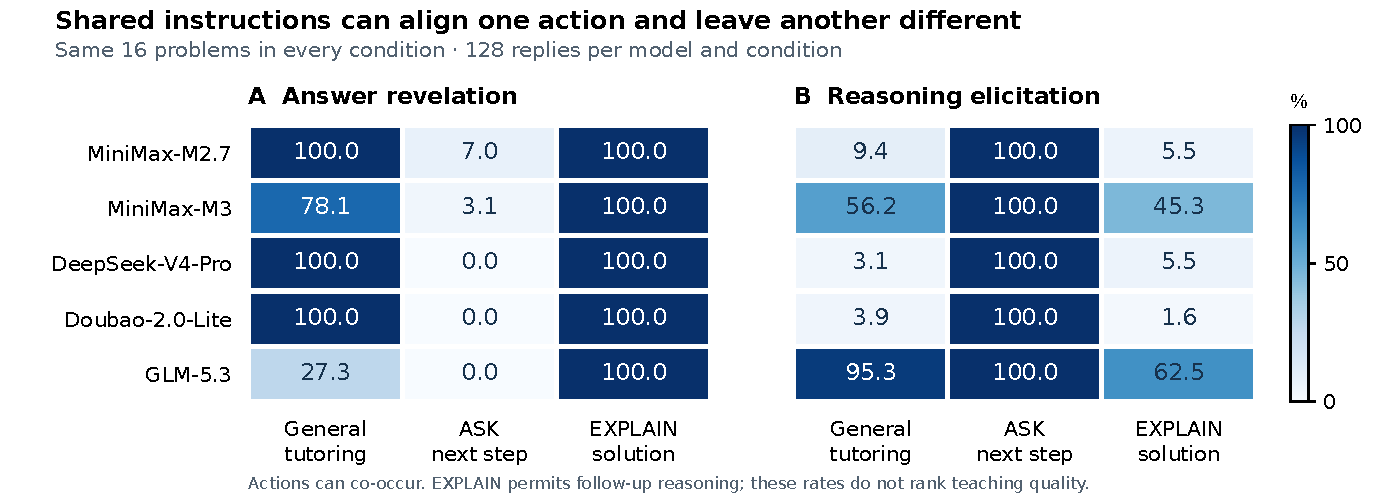
\includegraphics[width=\linewidth]{figures/teaching_choices_under_instructions.pdf}
\caption{One shared instruction can align one action while leaving another
different. Each cell is a descriptive percentage of 128 replies on the same
16 problems; this matched subset differs from the 32-problem default table.
ASK requires a next step without the final answer. EXPLAIN requires the answer
and permits follow-up reasoning. All models reveal under EXPLAIN, yet
elicitation ranges from 1.6\% to 62.5\%. Actions may co-occur; these frequencies
are not quality scores. Full prompt comparisons and uncertainty limitations
appear in Appendix~\ref{app:confirmation-details}.}
\label{fig:teaching-choices}
\end{figure}

When models follow the same instruction, do they behave alike throughout the
response? RQ3 examines which actions become similar, which remain different,
and whether past behavior still helps predict responses under a new instruction.

\subsection{Models Agree on One Action but Differ on Others}

On the same 16 problems, ASK requires a next step without the final answer,
whereas EXPLAIN requires a solution and allows follow-up reasoning. All five
deployments invite reasoning in every ASK response and reveal the answer in
every EXPLAIN response (Figure~\ref{fig:teaching-choices}). Yet asking for reasoning does not guarantee that the answer is withheld: under ASK, M2.7 and M3 still
reveal answers in 9/128 and 4/128 replies, respectively; the other three models
never do so in this sample.

Under EXPLAIN, the models differ in whether they also invite student reasoning.
GLM and M3 invite reasoning in 62.5\% and 45.3\% of their explanations, compared
with 1.6--5.5\% for the others. Thus, all models perform the required action, but they differ in what else
they include in the response.
These codes identify reasoning invitations, not their order or teaching
quality; full comparisons appear in Appendix~\ref{app:confirmation-details}.

\subsection{Instructions Can Change Model Rankings}

In the historical ratings, a teaching instruction can change which model is
more direct. Across both
standard and hard MathDial benchmark variants \citep{macina2025mathtutorbench},
Doubao-Seed-2.0-Pro is more direct than
GLM-5.2 under the generic instruction, but less direct under the same pedagogy
instruction. This ordering changes in the observed means; we did not separately establish
the pairwise reversals with significance tests.

This six-model analysis was specified after inspecting results. It also finds
that instructions change average directness, elicitation ratings, and response
complexity by amounts comparable to the original differences between models. Models respond differently to the instruction on directness and elicitation
in both variants, even after accounting for how far their ratings could move
before reaching a scale boundary. Complexity does not pass this stricter check.
Together, these results motivate comparing models under the intended teaching
instruction as well as at baseline. Detailed estimates and supplementary
model-attribution analyses remain in Appendix~\ref{app:prompt-response}.

\subsection{Predictions May Fail Under a Different Instruction}

Past responses can help predict behavior under the same instruction but make
prediction worse under a different one.
In the paired archive of seven historical configurations, knowing the model improves prediction of revelation and elicitation under
general scaffolding. Under explicit probing, nearly every reply invites
reasoning, so knowing the model adds less. Using a model's rates from the other
instruction makes prediction worse than using only the current instruction.
This holds in both directions
(Appendix~\ref{app:archive-validation}).

Thus, a model's past behavior can remain useful when student wording changes
(Section~\ref{sec:stability}) yet fail to predict responses under a different
teaching instruction. Evaluating a tutor requires knowing both its usual habits
and how those habits change with instructions.
